%%%%%%%%%%%%%%%%%%%%%%%%%%%%%%%%%%%%%%%%%
% Beamer Presentation
% LaTeX Template
% Version 1.0 (10/11/12)
%
% This template has been downloaded from:
% http://www.LaTeXTemplates.com
%
% License:
% CC BY-NC-SA 3.0 (http://creativecommons.org/licenses/by-nc-sa/3.0/)
%
%%%%%%%%%%%%%%%%%%%%%%%%%%%%%%%%%%%%%%%%%

%----------------------------------------------------------------------------------------
%	PACKAGES AND THEMES
%----------------------------------------------------------------------------------------

\documentclass{beamer}

\mode<presentation> {

% The Beamer class comes with a number of default slide themes
% which change the colors and layouts of slides. Below this is a list
% of all the themes, uncomment each in turn to see what they look like.

%\usetheme{default}
%\usetheme{AnnArbor}
%\usetheme{Antibes}
%\usetheme{Bergen}
%\usetheme{Berkeley}
%\usetheme{Berlin}
%\usetheme{Boadilla}
%\usetheme{CambridgeUS}
%\usetheme{Copenhagen}
%\usetheme{Darmstadt}
%\usetheme{Dresden}
%\usetheme{Frankfurt}
%\usetheme{Goettingen}
%\usetheme{Hannover}
%\usetheme{Ilmenau}
%\usetheme{JuanLesPins}
%\usetheme{Luebeck}
\usetheme{Madrid}
%\usetheme{Malmoe}
%\usetheme{Marburg}
%\usetheme{Montpellier}
%\usetheme{PaloAlto}
%\usetheme{Pittsburgh}
%\usetheme{Rochester}
%\usetheme{Singapore}
%\usetheme{Szeged}
%\usetheme{Warsaw}

% As well as themes, the Beamer class has a number of color themes
% for any slide theme. Uncomment each of these in turn to see how it
% changes the colors of your current slide theme.

%\usecolortheme{albatross}
%\usecolortheme{beaver}
%\usecolortheme{beetle}
%\usecolortheme{crane}
%\usecolortheme{dolphin}
%\usecolortheme{dove}
%\usecolortheme{fly}
%\usecolortheme{lily}
%\usecolortheme{orchid}
%\usecolortheme{rose}
%\usecolortheme{seagull}
%\usecolortheme{seahorse}
%\usecolortheme{whale}
%\usecolortheme{wolverine}

%\setbeamertemplate{footline} % To remove the footer line in all slides uncomment this line
%\setbeamertemplate{footline}[page number] % To replace the footer line in all slides with a simple slide count uncomment this line

%\setbeamertemplate{navigation symbols}{} % To remove the navigation symbols from the bottom of all slides uncomment this line
}

\usepackage{graphicx} % Allows including images
\usepackage{booktabs} % Allows the use of \toprule, \midrule and \bottomrule in tables

%----------------------------------------------------------------------------------------
%	TITLE PAGE
%----------------------------------------------------------------------------------------

\title[Anum - SPL]{Analisis Numerik\\Solusi Sistem Persamaan Linier} % The short title appears at the bottom of every slide, the full title is only on the title page

\author{Ahmad Rio Adriansyah} % Your name
\institute[STTT-NF] % Your institution as it will appear on the bottom of every slide, may be shorthand to save space
{
STT Terpadu - Nurul Fikri \\ % Your institution for the title page
\medskip
\textit{ahmad.rio.adriansyah@gmail.com\\arasy@nurulfikri.ac.id} % Your email address
}
\date{} % Date, can be changed to a custom date

\usepackage{amsmath}
\usepackage{graphicx}
\begin{document}

\begin{frame}
\titlepage % Print the title page as the first slide
\end{frame}

%----------------------------------------------------------------------------------------
%	PRESENTATION SLIDES
%----------------------------------------------------------------------------------------

%------------------------------------------------

\begin{frame}
\frametitle{Sistem Persamaan Linier}
\begin{itemize}
\item Persamaan linier = Persamaan yang hanya mengandung konstanta dan peubah dengan pangkat tertinggi 1
\item Sistem persamaan linier = Sejumlah persamaan linier yang harus diselesaikan secara simultan
\end{itemize}
\end{frame}

%------------------------------------------------

\begin{frame}
\frametitle{SPL dengan 2 Peubah}
Contoh : 
\begin{equation}
\Biggl\{ \begin{matrix}2x+y=&1\\x+2y=&-4\end{matrix}
\nonumber
\end{equation}
Cara pernyelesaian :
\begin{itemize}
\item Metode Substitusi
\item Metode Eliminasi
\item Metode Gabungan (substitusi dan eliminasi)
\end{itemize}
\end{frame}

%------------------------------------------------

\begin{frame}
\frametitle{Metode Substitusi}
\begin{itemize}
\item Satu persamaan diatur agar hanya ada 1 peubah di sebelah kiri
\begin{equation}
y= 1-2x
\nonumber
\end{equation}
\item Substitusikan peubah tersebut ke dalam persamaan yang lainnya
\begin{equation}
\begin{split}
x+ 2(1-2x)&=-4
\\x+2-4x&=-4
\\x-4x&=-4-2
\\-3x&=-6
\\x&=2
\end{split}
\nonumber
\end{equation}
\item Substitusikan nilai peubah yang sudah didapat ke persamaan asal
\begin{equation}
\begin{split}
y&= 1-2(2) = 1-4 
\\y&=-3
\end{split}
\nonumber
\end{equation}
\end{itemize}
\end{frame}

%------------------------------------------------

\begin{frame}
\frametitle{Metode Eliminasi}

\begin{itemize}
\item Samakan koefisien salah satu peubah
\begin{equation}
\Biggl\{ \begin{matrix}2x+y=&1 &\times 1\\x+2y=&-4& \times 2\end{matrix} \quad \rightarrow 
\Biggl\{ \begin{matrix}2x+y=&1 \\2x+4y=&-8\end{matrix}
\nonumber
\end{equation}
\item Eliminasi salah satu peubah
\begin{equation}
\begin{matrix}2x+y&=&1 \\2x+4y&=&-8 & -\\\hline \\-3y &=& 9\end{matrix}
\nonumber
\end{equation}
\begin{equation}
\boxed{y=-3}
\nonumber
\end{equation}
\item Lakukan hal yang sama untuk peubah lainnya
\end{itemize}
\end{frame}

%------------------------------------------------

\begin{frame}
\frametitle{SPL dengan 3 Peubah}
Contoh : 
\begin{equation}
\Biggl\{ \begin{matrix}x+y+z=&6\\2x+y-z=&1\\x-y+z=&2\end{matrix}
\nonumber
\end{equation}
atau
\begin{equation}
\Biggl\{ \begin{matrix}3x_1-2x_2+x_3=&0\\2x_1+x_2+3x_3=&13\\x_1-x_2-2x_3=&-7\end{matrix}
\nonumber
\end{equation}
\end{frame}

%------------------------------------------------

\begin{frame}
\frametitle{Bentuk Umum SPL}
Sistem persamaan linier dengan $n$ peubah dapat dinyatakan sebagai
\begin{center}
$\begin{matrix}
	a_{11}x_1+a_{12}x_2+\dots + a_{1n}x_n & =b_1\\
	a_{21}x_1+a_{22}x_2+\dots + a_{2n}x_n & =b_2\\
	\vdots & \vdots \\
	a_{n1}x_1+a_{n2}x_2+\dots + a_{nn}x_n & =b_n
\end{matrix}$
\end{center}
\ \\dengan \\$a_{ij}, b_i$ konstan, \\$x_i$ peubah \\untuk $i,j=1,2,\dots n$
\end{frame}

%------------------------------------------------

\begin{frame}
\frametitle{Bentuk Umum SPL}
dan dapat dituliskan dalam bentuk persamaan matriks
\begin{equation}
Ax=b
\nonumber
\end{equation}
dimana \\\ \\
$A=\begin{bmatrix}
	a_{11} & a_{12} & a_{13} & \dots & a_{1n}\\
	a_{21} & a_{22} & a_{23} & \dots & a_{2n}\\
	a_{31} & a_{32} & a_{33} & \dots & a_{3n}\\
	 & \vdots &  & \ddots & \vdots\\
	a_{n1} & a_{n2} & a_{n3} & \dots & a_{nn}\\
\end{bmatrix}, \quad x=\begin{bmatrix}x_1\\x_2\\x_3\\\vdots\\x_n\end{bmatrix}, \quad b=\begin{bmatrix}b_1\\b_2\\b_3\\\vdots\\b_n\end{bmatrix}$

\end{frame}

%------------------------------------------------

\begin{frame}
\frametitle{Penyulihan Mundur}
Jika matriks $A$ berbentuk matriks segitiga atas sehingga sistem persamaannya menjadi
\begin{center}
$\begin{bmatrix}
	a_{11} & a_{12} & a_{13} & \dots & a_{1n}\\
	0 & a_{22} & a_{23} & \dots & a_{2n}\\
	0 & 0 & a_{33} & \dots & a_{3n}\\
	 & \vdots &  & \ddots & \vdots\\
	0 & 0 & 0 & \dots & a_{nn}\\
\end{bmatrix}\begin{bmatrix}x_1\\x_2\\x_3\\\vdots\\x_n\end{bmatrix}=\begin{bmatrix}b_1\\b_2\\b_3\\\vdots\\b_n\end{bmatrix}$
\end{center}
\ \\solusi dapat diperoleh dengan cara penyulihan mundur (\textit{backward substitution})
\end{frame}

%------------------------------------------------

\begin{frame}
\frametitle{Penyulihan Mundur}
\begin{figure}[htp]
\centering
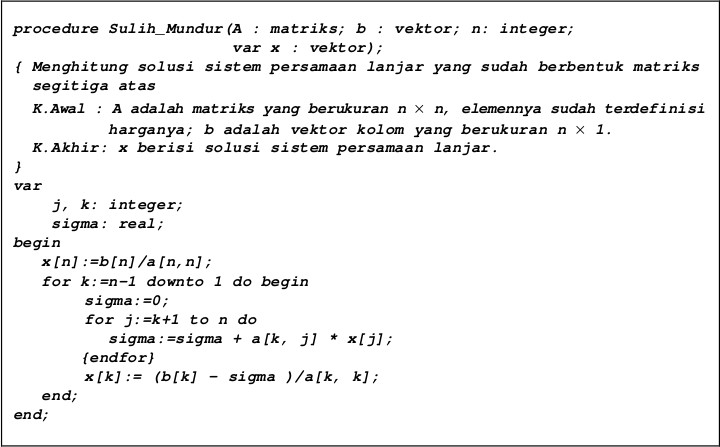
\includegraphics[scale=0.45]{sulihmundur.jpg}
\end{figure}\end{frame}

%------------------------------------------------

\begin{frame}
\frametitle{Penyulihan Mundur}
\begin{equation}
\begin{split}
a_{nn}x_n = b_n &\rightarrow x_n = b_n/a_{nn}
\\a_{_{n-1,n-1}}x_{n-1}+a_{_{n-1,n}}x_n = b_{n-1} &\rightarrow x_{n-1} = \dfrac{b_{n-1}-a_{_{n-1,n}}x_n}{a_{_{n-1,n-1}}}
\\&\vdots
\\&dst
\end{split}
\nonumber
\end{equation}
Jika $x_n,x_{n-1},x_{n-2},\dots,x_{k+1}$ diketahui, maka $x_k$ dapat dihitung dengan 
\begin{equation}
x_k = \dfrac{b_k - \sum_{j=k+1}^n{(a_{kj}x_j)}}{a_{kk}}
\nonumber
\end{equation}
untuk $k=n-1,n-2,\dots, 1$ dan $a_{kk} \neq 0$
\end{frame}

%------------------------------------------------

\begin{frame}
\frametitle{Eliminasi Gauss}
Tujuannya untuk mengubah matriks $A$ pada persamaan matriks $Ax=b$ menjadi matriks segitiga atas. 
\begin{equation}
Ax=b \rightarrow Ux=c
\nonumber
\end{equation}
dimana $U$ adalah matriks segitiga atas $n\times n$, dan  $x,c$ matriks kolom berukuran $n$.
\\\ \\Mengubahnya dengan menggunakan "operasi baris elementer" (OBE).
\\\ \\OBE mengubah persamaan, tetapi tidak mengubah solusi dari sistem persamaannya.
\end{frame}

%------------------------------------------------

\begin{frame}
\frametitle{OBE}
Terdiri dari 3 buah operasi :
\begin{itemize}
\item Pertukaran : Menukar urutan dua buah persamaan
\item Penskalaan : Mengalikan sebuah persamaan dengan konstanta tak nol
\item Penjumlahan : Mengganti sebuah persamaan dengan penjumlahan persamaan itu dengan persamaan lain.
\end{itemize}
\end{frame}

%------------------------------------------------

\begin{frame}
\frametitle{OBE}
Contoh :
\begin{center}
$\Biggl\{\begin{matrix}
	2x_1+3x_2-x_3 & =5\\
	4x_1+4x_2-3x_3 & =3\\
	-2x_1+3x_2-x_3 & =1\\
\end{matrix}$
\end{center}
Sistem persamaan tersebut dapat diubah menjadi bentuk persamaan matriks
\begin{equation}
\begin{bmatrix}
	2 & 3 & -1\\
	4 & 4 & -3\\
	-2 & 3 & -1\\
\end{bmatrix}
\begin{bmatrix}
	x_1\\
	x_2\\
	x_3\\
\end{bmatrix}=
\begin{bmatrix}
	5\\
	3\\
	1\\
\end{bmatrix}
\nonumber
\end{equation}
Untuk melakukan OBE, persamaan matriks tersebut dapat kita buat menjadi bentuk yang tergabung
\begin{equation}
\begin{bmatrix}
	2 & 3 & -1 &| &5\\
	4 & 4 & -3&| &3\\
	-2 & 3 & -1&| &1\\
\end{bmatrix}
\nonumber
\end{equation}

\end{frame}
%------------------------------------------------

\begin{frame}
\frametitle{OBE}
\begin{equation}
\begin{split}
\begin{bmatrix}
	2 & 3 & -1 &| &5\\
	4 & 4 & -3&| &3\\
	-2 & 3 & -1&| &1\\
\end{bmatrix} &\sim^{R_3+R_1 \rightarrow R_3}\sim 
\begin{bmatrix}
	2 & 3 & -1 &| &5\\
	4 & 4 & -3&| &3\\
	0 & 6 & -2&| &6\\
\end{bmatrix}
\\&\sim^{R_2-2R_1 \rightarrow R_2}\sim 
\begin{bmatrix}
	2 & 3 & -1 &| &5\\
	0 & -2 & -1&| &-7\\
	0 & 6 & -2&| &6\\
\end{bmatrix}
\\&\sim^{R_3+3R_2 \rightarrow R_3}\sim 
\begin{bmatrix}
	2 & 3 & -1 &| &5\\
	0 & -2 & -1&| &-7\\
	0 & 0 & -5&| &-15\\
\end{bmatrix}
\end{split}
\nonumber
\end{equation}

\end{frame}


%------------------------------------------------

\begin{frame}
\frametitle{Latihan}
Ubahlah sistem persamaan linier berikut menjadi bentuk persamaan matriks, dan ubah matriksnya menjadi matriks segitiga atas dengan Eliminasi Gauss.
\begin{center}
$1\quad \Biggl\{\begin{matrix}
	x_1+2x_2+x_3 & =-1\\
	3x_1+6x_2-x_3 & =1\\
	-x_1+x_2+x_3 & =-3\\
\end{matrix}$
\\\ \\\ \\
$2\quad \Biggl\{\begin{matrix}
	x_1+x_2+x_3 & =1\\
	2x_1+3x_2+x_3 & =4\\
	3x_1+x_2+2x_3 & =2\\
\end{matrix}$
\end{center}

\end{frame}
%------------------------------------------------

\begin{frame}
\frametitle{Eliminasi Gauss}
Nilai $a_{r,r}$ yang digunakan untuk mengeliminasi $x_r$ pada baris ke $r+1,r+2, \dots, n$ disebut elemen \underline{pivot} dan persamaan pada baris ke-$r$ disebut \underline{persamaan pivot}.
\\\ \\
Elemen pivot dapat bernilai nol sehingga bisa terjadi pembagian dengan nol. Metode eliminasi yang tidak memperdulikan kemungkinan ini disebut dengan \underline{Eliminasi Gauss Naif}. Naif karena metodenya tidak melakukan pemeriksaan kemungkinan pembagian dengan nol.
\\\ \\Untuk menghindari elemen pivot yang bernilai nol, dapat dilakukan operasi pertukaran baris. Metode ini disebut sebagai \underline{Eliminasi Gauss dengan Pivoting}
\end{frame}

%------------------------------------------------

\begin{frame}
\frametitle{Eliminasi Gauss dengan Pivoting}
Contoh : \\\ \\
\begin{center}$\Biggl\{$\begin{tabular}{ll}
	$x_1+2x_2+x_3$ & $=2$\\
	$3x_1+6x_2$ & $=9$\\
	$2x_1+8x_2+4x_3$ & $=6$\\
\end{tabular}
\end{center}
Sistem persamaan tersebut dapat diubah menjadi bentuk persamaan matriks
\begin{equation}
\begin{bmatrix}
	1 & 2 & 1\\
	3 & 6 & 0\\
	2 & 8 & 4\\
\end{bmatrix}
\begin{bmatrix}
	x_1\\
	x_2\\
	x_3\\
\end{bmatrix}=
\begin{bmatrix}
	2\\
	9\\
	6\\
\end{bmatrix}
\nonumber
\end{equation}
Untuk melakukan OBE, persamaan matriks tersebut dapat kita buat menjadi bentuk yang tergabung
\begin{equation}
\begin{bmatrix}
	1 & 2 & 1 & | & 2\\
	3 & 6 & 0& | & 9\\
	2 & 8 & 4 & | & 6\\
	\end{bmatrix}
\nonumber
\end{equation}

\end{frame}

%------------------------------------------------

\begin{frame}
\frametitle{OBE}
\begin{equation}
\begin{split}
\begin{bmatrix}
	1 & 2 & 1 & | & 2\\
	3 & 6 & 0& | & 9\\
	2 & 8 & 4 & | & 6\\
	\end{bmatrix} \sim^{R_2+3R_1 \rightarrow R_2}\sim 
&\begin{bmatrix}
	1 & 2 & 1 &| &2\\
	0 & 0 & -3&| &3\\
	2 & 8 & 4&| &6\\
\end{bmatrix}
\\\sim^{R_3-2R_1 \rightarrow R_3}\sim 
&\begin{bmatrix}
	1 & 2 & 1 &| &2\\
	0 & 0 & -3&| &3\\
	0 & 4 & 2&| &2\\
\end{bmatrix}
\\\sim^{R_3\leftrightarrow R_2}\sim 
&\begin{bmatrix}
	1 & 2 & 1 &| &2\\
	0 & 4 & 2&| &2\\
	0 & 0 & -3&| &3\\
\end{bmatrix}
\end{split}
\nonumber
\end{equation}

\end{frame}

%------------------------------------------------

\begin{frame}
\frametitle{Penyulihan Mundur}
Setelah didapat matriks segitiga atas, maka dapat dilakukan penyulihan mundur untuk mendapatkan solusi.
\begin{equation}
\begin{bmatrix}
	1 & 2 & 1 &| &2\\
	0 & 4 & 2&| &2\\
	0 & 0 & -3&| &3\\
\end{bmatrix} \longrightarrow 
\begin{bmatrix}
	1 & 2 & 1\\
	0 & 4 & 2\\
	0 & 0 & -3\\
\end{bmatrix}\begin{bmatrix}
	x_1\\
	x_2\\
	x_3\\
\end{bmatrix}=\begin{bmatrix}
	2\\
	2\\
	3\\
\end{bmatrix}
\nonumber
\end{equation}
\begin{equation}
\begin{split}
-3x_3 = 3 &\rightarrow x_3=\dfrac{3}{-3}=\boxed{-1}
\\4x_2+2x_3=2 &\rightarrow 4x_2-2=2 \\&\rightarrow x_2=\dfrac{4}{4} = \boxed{1}
\\x_1+2x_2+x_3=2 &\rightarrow x_1+2-1=2
\\&\rightarrow x_1=\boxed{1}
\end{split}
\nonumber
\end{equation}

\end{frame}


%------------------------------------------------

\begin{frame}
\frametitle{Mengurangi Galat}
Tata Ancang \textit{pivoting}
\begin{itemize}
\item Pivoting sebagian (\textit{partial pivoting})
\\Pivot dipilih dari semua elemen pada kolom $p$ yang mempunyai nilai mutlak terbesar
\\
\begin{equation}
\begin{bmatrix}
	x & x & x & x & | & x\\
	0 & \boxed{x} & x & x & | & x\\
	0 & \boxed{x} & x & x & | & x\\
	0 & \boxed{x} & x & x & | & x\\
\end{bmatrix}
\nonumber
\end{equation}
\ \\\begin{small}*dicari nilai $|x|$ terbesar lalu barisnya dipertukarkan dengan baris kedua\end{small}
\item Pivoting lengkap (\textit{complete pivoting})
\\Disamping baris, kolom juga diikutkan dalam pencarian elemen terbesar dan dipertukarkan.
\end{itemize}
\end{frame}

%------------------------------------------------

\begin{frame}
\frametitle{Mengurangi Galat}
Contoh : 
\\\begin{center}
$\Biggl\{\begin{matrix}
	3x_1-0.1x_2-0.2x_3 & =&7.85\\
	0.3x_1-0.2x_2+10x_3 & =&71.4\\
	0.1x_1+7x_2-0.3x_3 & =&-19.3\\
\end{matrix}$
\end{center}
Solusi eksaknya adalah $x_1=3,\ x_2=-2.5,$ dan $x_3=7$
\\Perhitungan akan dilakukan dengan 4 digit di belakang koma.
\end{frame}

%------------------------------------------------

\begin{frame}
\frametitle{Tanpa Pivoting}
\begin{small}
\begin{equation}
\begin{split}
\begin{bmatrix}
	3 & -0.1 & -0.2 & | & 7.85\\
	0.3 & -0.2 & 10 & | & 71.4\\
	0.1 & 7 & -0.3 & | & -19.3\\
	\end{bmatrix}&\\ \sim^{R_1+30R_3 \rightarrow R_3}\sim 
&\begin{bmatrix}
	3 & -0.1 & -0.2 & | & 7.85\\
	0.3 & -0.2 & 10 & | & 71.4\\
	0 & -210.1 & 8.8 & | & 586.85\\
\end{bmatrix}
\\\sim^{R_1-10R_2 \rightarrow R_2}\sim 
&\begin{bmatrix}
	3 & -0.1 & -0.2 & | & 7.85\\
	0 & 1.9 & -100.2 & | & -706.15\\
	0 & -210.1 & 8.8 & | & 586.85\\
\end{bmatrix}
\\\sim^{R_3*(1.9/-210.1)}\sim 
&\begin{bmatrix}
	3 & -0.1 & -0.2 & | & 7.85\\
	0 & 1.9 & -100.2 & | & -706.15\\
	0 & 1.9 & -0.0796 & | & -5.3071\\
\end{bmatrix}
\\\sim^{R_3-R_2 \rightarrow R_3)}\sim 
&\begin{bmatrix}
	3 & -0.1 & -0.2 & | & 7.85\\
	0 & 1.9 & -100.2 & | & -706.15\\
	0 & 0 & 100.1204 & | & 700.8429\\
\end{bmatrix}
\end{split}
\nonumber
\end{equation}
\end{small}
\end{frame}

%------------------------------------------------
\begin{frame}
\frametitle{Tanpa Pivoting}
\begin{equation}
\begin{split}
100.1204x_3 = 700.8429 \qquad&\rightarrow x_3=\boxed{7.0000009988}
\\1.9x_2-100.2x_3=-706.15 \  &\rightarrow x_2=\boxed{-2.4999473266}
\\3x_1-0.1x_2-0.2x_3=7.85 \  &\rightarrow x_1=\boxed{3.0000018224}
\end{split}
\nonumber
\end{equation}
Galat perhitungan adalah selisih nilai eksak dan nilai perhitungan\\$\epsilon=x_{hitung}-x_{eksak}$ 
\begin{equation}
\begin{split}
\epsilon_{x_1}=& 3.0000018224-3 = 0.0000018224
\\\epsilon_{x_2}=& (-2.4999473266)-(-2.5) = 0.0000526734
\\\epsilon_{x_3}=& 7.0000009988-7 = 0.0000009988
\end{split}
\nonumber
\end{equation}

\end{frame}

%------------------------------------------------
\begin{frame}
\frametitle{Dengan Pivoting}
\begin{small}
\begin{equation}
\begin{split}
\begin{bmatrix}
	\boxed{3} & -0.1 & -0.2 & | & 7.85\\
	0.3 & -0.2 & 10 & | & 71.4\\
	0.1 & 7 & -0.3 & | & -19.3\\
	\end{bmatrix}&\\ \sim^{R_1+30R_3 \rightarrow R_3}\sim 
&\begin{bmatrix}
	3 & -0.1 & -0.2 & | & 7.85\\
	0.3 & -0.2 & 10 & | & 71.4\\
	0 & -210.1 & 8.8 & | & 586.85\\
\end{bmatrix}
\\\sim^{R_1-10R_2 \rightarrow R_2}\sim 
&\begin{bmatrix}
	3 & -0.1 & -0.2 & | & 7.85\\
	0 & 1.9 & -100.2 & | & -706.15\\
	0 & \boxed{-210.1} & 8.8 & | & 586.85\\
\end{bmatrix}
\\\sim^{R_2\leftrightarrow R_3}\sim 
&\begin{bmatrix}
	3 & -0.1 & -0.2 & | & 7.85\\
	0 & -210.1 & 8.8 & | & 586.85\\
	0 & 1.9 & -100.2 & | & -706.15\\
\end{bmatrix}
\\\sim^{R_2+\frac{210.1}{1.9}R_3 \rightarrow R_3)}\sim 
&\begin{bmatrix}
	3 & -0.1 & -0.2 & | & 7.85\\
	0 & -210.1 & 8.8 & | & 586.85\\
	0 & 0 & -11071.2105 & | & -77498.4737\\
\end{bmatrix}
\end{split}
\nonumber
\end{equation}
\end{small}
\end{frame}

%------------------------------------------------
\begin{frame}
\frametitle{Dengan Pivoting}
\begin{equation}
\begin{split}
-11071.2105x_3 = -77498.4737 \qquad&\rightarrow x_3=\boxed{7.0000000181}
\\-210x_2+8.8x_3=586.85 \  &\rightarrow x_2=\boxed{-2.4999999992}
\\3x_1-0.1x_2-0.2x_3=7.85 \  &\rightarrow x_1=\boxed{3.0000000012}
\end{split}
\nonumber
\end{equation}
Galat perhitungannya
\\$\epsilon=x_{hitung}-x_{eksak}$ 
\begin{equation}
\begin{split}
\epsilon_{x_1}=& 3.0000000012-3 = 0.0000000012
\\\epsilon_{x_2}=& (-2.4999999992)-(-2.5) = 0.0000000008
\\\epsilon_{x_3}=& 7.0000000181-7 = 0.0000000181
\end{split}
\nonumber
\end{equation}

\end{frame}

%------------------------------------------------

\begin{frame}
\frametitle{Galat}
Galat mutlak adalah nilai mutlak dari selisih nilai eksak dan nilai perhitungan
\\$\epsilon=|x_{hitung}-x_{eksak}|$
\\\ \\Galat mutlaknya
\begin{center}
\begin{tabular}{|l|l|l|}
\hline
	 & Tanpa Pivoting & Dengan Pivoting\\
\hline
	$x_1$ & 0.0000018224 & 0.0000000012\\
\hline  
	$x_2$ & 0.0000526734 & 0.0000000008\\
\hline
	$x_3$ & 0.0000009988 & 0.0000000181\\
\hline
\end{tabular}
\end{center}
\end{frame}

%------------------------------------------------

\begin{frame}
\frametitle{Mengurangi Galat}
Penskalaan (\textit{scaling})
\\Penskalaan digunakan untuk SPL \textbf{yang mempunyai perbedaan koefisien yang mencolok}. Caranya adalah dengan membagi tiap baris persamaan dengan nilai mutlak koefisien terbesar di ruas kirinya sehingga koefisien maksimum dalam tiap baris adalah 1.
\\\ \\Contoh :
\\\ \\$\begin{bmatrix}
	2 & 100000 & | & 100000\\
	1 & 1 & | & 2\\
\end{bmatrix} \sim \begin{bmatrix}
	2 & 100000 & | & 100000\\
	0 & -49999 & | & -49998\\
\end{bmatrix}$
\\\ \\Jika kita menggunakan perhitungan dengan 4 angka di belakang koma, maka persamaan tersebut menghasilkan solusi yang salah $x_1=0, x_2=1$
\end{frame}

%------------------------------------------------

\begin{frame}
\frametitle{Mengurangi Galat}
Namun jika kita skalakan terlebih dahulu
\\\ \\$\begin{bmatrix}
	2 & 100000 & | & 100000\\
	1 & 1 & | & 2\\
\end{bmatrix}\sim \begin{bmatrix}
	0.00002 & 1 & | & 1\\
	1 & 1 & | & 2\\
\end{bmatrix}\sim \begin{bmatrix}
	1 & 1 & | & 2\\
	0.00002 & 1 & | & 1\\
\end{bmatrix}$
\\\ \\\ \\$\sim \begin{bmatrix}
	1 & 1 & | & 2\\
	0 & 1 & | & 1\\
\end{bmatrix}$
\\\ \\perhitungannya memberikan solusi yang benar $x_1=x_2=1$
\end{frame}

%------------------------------------------------

\begin{frame}
\frametitle{Kemungkinan Solusi SPL}
\begin{itemize}
\item Solusi unik
\\Jika pada hasil eliminasi Gauss tidak terdapat baris yang semuanya bernilai 0
\item Banyak solusi
\\Jika pada hasil eliminasi Gauss terdapat setidaknya satu baris yang semuanya 0
\item Tidak ada solusi
\\Jika pada hasil eliminasi Gauss terdapat baris yang semuanya bernilai 0, tetapi elemen pada baris yang bersesuaian di vektor kolom b tidak 0
\end{itemize}
\end{frame}


%------------------------------------------------

\begin{frame}
\frametitle{Metode Iterasi}
Penggunaan metode eliminasi Gauss mengakibatkan banyak galat pembulatan sehingga solusi yang diperoleh bisa jauh dari solusi sebenarnya.
\\\ \\Untuk mengatasinya, dapat digunakan metode iterasi. Dengan metode ini, galat pembulatan dapat diperkecil karena kita dapat melanjutkan iterasi sampai didapat solusi seteliti mungkin.
\\\ \\Metode eliminasi Gauss disebut metode langsung dan metode yang menggunakan iterasi disebut metode tak langsung.
\end{frame}

%------------------------------------------------

\begin{frame}
\frametitle{Metode Iterasi}
Sistem persamaan linier 
\begin{center}
$\begin{matrix}
	a_{11}x_1+a_{12}x_2+\dots + a_{1n}x_n & =b_1\\
	a_{21}x_1+a_{22}x_2+\dots + a_{2n}x_n & =b_2\\
	\vdots & \vdots \\
	a_{n1}x_1+a_{n2}x_2+\dots + a_{nn}x_n & =b_n
\end{matrix}$
\end{center}
dapat diselesaikan dengan iterasi dengan syarat $a_{kk}\neq 0$
\\\ \\$x_i^{(k)}$ maksudnya adalah nilai dari peubah $x_i$ pada iterasi ke $k$
\end{frame}

%------------------------------------------------

\begin{frame}
\frametitle{Metode Iterasi}
Persamaan iterasinya dapat ditulis sebagai berikut
\begin{equation}
\begin{split}
x_1^{(k+1)} &=\dfrac{b_1-a_{12}x_2^{(k)}-a_{13}x_3^{(k)}-...-a_{1n}x_n^{(k)}}{a_{11}}
\\x_2^{(k+1)} &=\dfrac{b_2-a_{21}x_1^{(k)}-a_{23}x_3^{(k)}-...-a_{2n}x_n^{(k)}}{a_{22}}
\\&\vdots
\\x_n^{(k+1)} &=\dfrac{b_n-a_{n1}x_1^{(k)}-a_{n2}x_2^{(k)}-...-a_{n,(n-1)}x_{n-1}^{(k)}}{a_{nn}}
\end{split}
\nonumber
\end{equation}
\end{frame}

%------------------------------------------------

\begin{frame}
\frametitle{Metode Iterasi}
Dengan tebakan awal 
\begin{equation}
x^{(0)}=\begin{bmatrix}
	x_1^{(0)}\\
	x_2^{(0)}\\
	\vdots\\
	x_n^{(0)}\\
\end{bmatrix}
\nonumber
\end{equation}
dan kondisi pemberhentian dapat ditentukan dengan galat relatif atau banyaknya iterasi\\\ 
\begin{equation}
\Biggl| \dfrac{x_i^{(k+1)}-x_i^{(k)}}{x_i^{(k+1)}}\Biggr| < \epsilon
\nonumber
\end{equation}

\end{frame}

%------------------------------------------------

\begin{frame}
\frametitle{Metode Iterasi Jacobi}
Rumus umum
\begin{equation}
x_i^{(k+1)}=\dfrac{b_i-\sum_{j\neq i}a_{ij}x_j^{(k)}}{a_{ii}}
\nonumber
\end{equation}
\begin{itemize}
\item Dari tebakan awal dan persamaan pertama didapatkan nilai $x_1^{(1)}$
\item Dari tebakan awal dan persamaan kedua didapatkan nilai $x_2^{(1)}$
\item Setelah semua nilai $x_i^{(1)}$ didapat, dihitung nilai $x_i^{(2)}$
\item dst
\end{itemize}
\end{frame}

%------------------------------------------------

\begin{frame}
\frametitle{Metode Iterasi Gauss-Seidel}
Rumus umum
\begin{equation}
x_i^{(k+1)}=\dfrac{b_i-\sum_{j=1}^{i-1}a_{ij}x_j^{(k+1)}-\sum_{j=i+1}^{n}a_{ij}x_j^{(k)}}{a_{ii}}
\nonumber
\end{equation}
\begin{itemize}
\item Dari tebakan awal dan persamaan pertama didapatkan nilai $x_1^{(1)}$
\item Nilai $x_1^{(1)}$ digunakan dalam perhitungan  nilai $x_2^{(1)}$
\item Nilai $x_1^{(1)}$ dan $x_2^{(1)}$ digunakan dalam perhitungan  nilai $x_3^{(1)}$
\item dst
\end{itemize}
\end{frame}

%------------------------------------------------

\begin{frame}
\frametitle{Metode Iterasi}
\begin{center}
buka file Iterasi.ods
\end{center}
\end{frame}
%------------------------------------------------

\end{document} 